\documentclass[11pt,a4paper]{article}
\usepackage[utf8]{inputenc}
\usepackage[T1]{fontenc}
\usepackage{geometry}
\geometry{left=2.7cm,right=2.7cm,top=2.6cm,bottom=2.6cm}
\usepackage{lmodern,microtype,setspace}
\usepackage{graphicx,float,amsmath,amssymb,cite,listings,xcolor,booktabs,array,caption,subcaption,algorithm,algpseudocode,tikz,pgfplots,seqsplit}
\usepackage[hidelinks]{hyperref}
\pgfplotsset{compat=1.18}
\usetikzlibrary{shapes,arrows,positioning,fit,backgrounds,matrix,calc}
\onehalfspacing
\setlength{\parindent}{1.5em}
\setlength{\parskip}{0.15em}
\hypersetup{
  pdftitle={Privacy Lens: An Evidence-Bounded Android Privacy Review Framework, Revision 17},
  pdfauthor={Zhiheng Zhang}
}
\title{Privacy Lens: An Evidence-Bounded Android Privacy Review Framework with Governed Legal-Evidence Packs (Revision 17)}
\author{Zhiheng Zhang \\ Student ID: 54560484 \\ Supervisor: Richard Sinnott}
\date{August 2026}
\begin{document}
\maketitle
\begin{abstract}
\small\singlespacing
Mobile privacy-review tools face an evidence-to-decision gap: a permission observation can indicate activity, but it cannot by itself establish purpose, necessity, lawful basis, acquisition completeness, or legal compliance. When an interface suppresses these missing facts, a technically correct calculation can still produce an unreliable conclusion. This thesis addresses that gap through Privacy Lens, a local-first Android prototype that converts bounded permission-audit summaries into traceable prompts for human review.

Following a design-science method, the architecture treats provenance, temporal scope, missing context, and uncertainty as first-class evidence rather than treating a count as a legal verdict. A fail-closed engine rejects malformed records and unsafe temporal aggregation, isolates simulator data, and records the rule-pack version applied to each finding. The European Union General Data Protection Regulation provides the evaluated legal objective; jurisdiction-specific mappings remain outside the Android, repository, and interface layers through a replaceable pack contract.

The implemented product organises the review journey around Overview, Findings, and Settings. Findings remain on the device, Android backup and remote updates are disabled, the evaluated package has no network or sensitive runtime permission, and users can clear local evidence directly. Revision 15 added source-status and legal-evidence governance. Revision 16 exposed provenance and non-colour status structure through an editorial interface. Revision 17 adds a signal--missing-context--proportionate-action reading path, applies the same sequence inside expanded findings, discourages action based on one card, and discloses the effect and reversibility of a synthetic demonstration before execution.

Evaluation separates rule conformance, hostile admission, temporal behaviour, pack identity, legal-evidence completeness, release packaging, manifest facts, physical installation, rendered interface evidence, and human-factors design contracts. In a fixed-seed 1,000-case corpus, the engine produced 800 true positives and 200 true negatives without disagreement against the specified threshold oracle. A further 1,800 independently calculated pack cases, basis-specific and DPIA evidence probes, governance mutations, strengthened accessibility contracts, and release-privacy contracts passed. The 1.5.0 ARM64 APK and AAB built successfully; the APK completed five final cold-start rounds on one OPPO PERM00 without a package-specific crash-buffer entry. Device captures covered the reading path, the finding reasoning sequence, the agency warning, and the pre-demonstration confirmation. No participant outcome is inferred from those rendered states.

These results establish an initial store-submission engineering candidate within the recorded scope. They do not establish legal compliance, unrestricted Android visibility, population accuracy, accessibility conformance, long-run reliability, or store approval. The contribution is an evidence-bounded architecture and traceability method that separate statutory motivation, engineering heuristics, observed evidence, missing legal facts, and prohibited conclusions.
\end{abstract}
\newpage
\tableofcontents
\newpage
\input{Iteration-V2/Chapter1/chapter-01-17}
\input{Iteration-V2/Chapter2/chapter-02-17}
\input{Iteration-V2/Chapter3/chapter-03-17}
\input{Iteration-V2/Chapter4/chapter-04-17}
\section{Evaluation and Results}

This chapter evaluates whether the implemented system preserves the evidence boundary defined in Chapters 2 and 3. The protocol separates logical conformance, hostile input handling, temporal state, pack identity, legal-evidence completeness, Android packaging, physical interaction, and visual communication. Results are reported before interpretation so that a positive engineering outcome is not silently promoted into a legal, population, or store-approval claim.

\subsection{Evaluation Overview and Headline Results}

The evaluation separates eight evidence layers: source conformance, deterministic rule behaviour, adversarial boundary behaviour, legal-evidence governance, Android package integration, physical-device behaviour, rendered-interface communication, and human-factors design contracts. This separation prevents a passed unit test from being reported as device reliability, human comprehension, or legal validity. Revision 17 renews the 1.5.0 artefacts and adds rendered checks for the reading path, finding reasoning sequence, agency warning, and pre-demonstration expectation disclosure.

\subsubsection{Source and Rule Verification}

The complete application passed \texttt{tsc --noEmit} and ESLint. The compliance sources were compiled before execution, preventing stale generated JavaScript from being treated as current evidence.

A fixed-seed logical campaign generated 1,000 cases. Eight hundred were expected review signals and 200 were below-threshold controls. The observed confusion matrix was

\begin{equation}
(TP,TN,FP,FN)=(800,200,0,0),
\end{equation}

which gives precision and recall of 1.0000 against the specified oracle. The oracle and engine implement the same published threshold model; this is a conformance and regression result, not an independent estimate of real-world infringement detection. Zero observed errors do not establish a zero population error rate.

Extended suites passed for unsafe types and integers, malformed context, unknown source, permission-key mutation, temporal overlap, adjacency, replay, retention, simulator isolation, dashboard presentation, missing-context disclosure, and regulation-pack identity. The tests confirm the enumerated boundaries. They cannot establish correctness for telemetry the application never receives or for legal interpretation outside the fixtures.

The retained deterministic campaign contains 1,800 cases across both packs and all three supported permission families. Its expected daily signal and threshold are calculated in a small reference function rather than by calling the production helper. Values at and immediately above each threshold confirm the strict comparison, while a fractional product confirms ceiling behaviour. Revision 15 extends governance mutations to impossible calendar dates, absence of a binding-law source, and explicit retention of consultation-material status. This improves oracle diversity and pack-contract coverage without turning generated cases into population evidence.

\subsubsection{Legal-Evidence Completeness Verification}

The legal tests now distinguish the six Article 6 bases instead of treating a selected enum value as complete evidence. Consent requires an Article 7 evidence reference; contract requires a necessity assessment; legal obligation and public task require an Article 6(3) mandate; vital interests requires a necessity assessment; and legitimate interests requires a three-part assessment. Cross-cutting probes require transparency, minimisation, retention justification, and a DPIA screening result. A positive DPIA screen without an assessment reference remains evidence-incomplete. Malformed new strings and Boolean fields fail with the same structured context error as earlier unsafe context.

These tests establish implementation of the declared question matrix, not legal sufficiency of the referenced records. The engine does not open, authenticate, or assess the legal reasoning in a reference. A withdrawn-consent observation is emitted as \texttt{POTENTIAL\_CONFLICT} with urgent review; the previous \texttt{LIKELY\_NON\_COMPLIANT} value is migration-only. This wording change reduces adjudicative overreach without asserting that every post-withdrawal access is unlawful, since timing, another legal basis, exceptions, and processing facts may still matter.

\subsubsection{Release Build and Manifest Verification}

Gradle completed \texttt{assembleRelease} and \texttt{bundleRelease} with target SDK 36. Table~\ref{tab:evaluated-artifacts} records the generated artefacts.

\begin{table}[H]
\centering
\small
\caption{Evaluated Android release artefacts}
\label{tab:evaluated-artifacts}
\begin{tabular}{p{0.31\textwidth}r p{0.42\textwidth}}
\toprule
Artefact & Bytes & SHA-256 \\
\midrule
\texttt{app-release.apk} & 59,411,247 & \texttt{\seqsplit{2ACE6B241FA515748A2473D68A0B23E51ABE90FDB071289EBEBBCA58B9871C9A}} \\
\texttt{app-release.aab} & 29,609,558 & \texttt{\seqsplit{A91F77AE8B8F7A38E0F41A5D5EB178F2828355791C1FD147776ECEC2E9DCABB2}} \\
\bottomrule
\end{tabular}
\end{table}

The 1.5.0 merged manifest contained wake lock, boot rescheduling, foreground service, and an app-scoped dynamic-receiver protection permission. Internet, network-state, and external-storage permissions were absent. Inspection confirmed application ID \path{com.zhihengzhang.privacylens}, version code 6, version name 1.5.0, minimum SDK 24, and target SDK 36. The signer remained the Android debug QA certificate rather than an owner-controlled production key.

\subsubsection{Physical-Device Evaluation}

The 1.5.0 networkless release APK was installed by ADB on one OPPO PERM00 device. Five force-stop and cold-start rounds completed. Median and mean \texttt{TotalTime} were 1,226 ms and 1,450.8 ms; sampled total PSS ranged from 98,347 to 100,743 KB; and the crash buffer contained no package-specific entry. Device captures covered the Overview reading path, expanded three-stage reasoning, the complete agency warning and legal caveat, and the pre-demonstration confirmation without obvious clipping or overlap in the inspected states. These are short-run observations, not a startup objective, participant comprehension, leak proof, legal validation, or broad performance claim.

The three primary destinations rendered at the device's captured application resolution. Coordinate-driven exploration initially appeared to show a navigation-target problem because the physical display and captured application coordinate spaces differed. A bounded coordinate sweep and UI-tree inspection identified the offset; subsequent navigation and custom bottom-bar interaction succeeded. This calibration episode is retained because it demonstrates why raw ADB coordinates must not be interpreted without the target's current window geometry.

The controlled demonstration completed a 50-record synthetic workflow. The populated overview displayed four review items, zero evidence gaps, two no-concern items, and descriptive precision and recall of 100\% for the simulator's known labels. The Findings screen marked the source as synthetic and displayed the EU GDPR pack. These values validate the demonstration path only; they are not device-observation accuracy.

\subsubsection{Usability and Trust Assessment}

The product was assessed against three release-candidate questions.

\begin{table}[H]
\centering
\small
\caption{Expert product-screening assessment}
\begin{tabular}{>{\raggedright\arraybackslash}p{0.19\textwidth}>{\raggedright\arraybackslash}p{0.32\textwidth}>{\raggedright\arraybackslash}p{0.37\textwidth}}
\toprule
Criterion & Supporting evidence & Boundary \\
\midrule
Visually coherent & consistent brand, hierarchy, spacing, cards, iconography, and three-destination navigation on the tested device & one device; no participant preference study \\
Trustworthy & local-first disclosure, source and pack labels, explicit missing evidence, no legal-verdict language & not a legal audit or security certification \\
Interaction feasibility & clear first action, concise summaries, optional details, demonstration, and direct data clearing & expert walkthrough only; no participant or longitudinal adoption measure \\
\bottomrule
\end{tabular}
\end{table}

The stricter publication-target rubric resets the predecessor App--thesis system to 70/100, assessed Revision 15 at 79/100, and assessed Revision 16 at 84/100. Under the same rubric, Revision 17 is assessed at 87/100: legal validity and governance 24/30, software evidence 23/25, interface and accessibility 19/20, user-psychology design evidence 13/15, and academic communication 8/10. The three-point movement reflects implemented expectation setting, uncertainty sequencing, proportional action, and reversible-demo disclosure. It does not award the remaining human-factors points because no participant task, comprehension, trust-calibration, or willingness-to-use result exists.

\subsection{Protocol and Reproducibility}

The protocol begins from six evaluation questions and assigns a separate acceptance condition to each. Reproducibility controls then ensure that the tests exercise current generated code, fixed temporal values, and explicit boundaries rather than relying on stale output or chance coverage.

\subsubsection{Evaluation Questions and Acceptance Logic}

The evaluation was organised around six questions. First, does the source compile and satisfy static rules? Second, does the decision engine agree with its specified thresholds and statuses? Third, does it reject malformed or adversarial evidence safely? Fourth, do regulation packs remain independent and traceable? Fifth, can the Android release artefacts be assembled, inspected, installed, and launched? Sixth, does the rendered product communicate the expected hierarchy and evidence boundaries on the available physical device?

Each question has a distinct acceptance condition. Source acceptance requires a clean TypeScript application check and ESLint run. Rule acceptance requires exact expected confusion-matrix values for the fixed corpus and passing boundary assertions. Runtime-boundary acceptance requires every malformed case to return the specified rejection code without an uncaught exception. Pack acceptance requires registry allowlisting, different thresholds where defined, retained pack identity, and a non-legal caveat for the Research Baseline.

Android build acceptance requires both release tasks to complete and the artefacts to exist with recorded hashes. Permission acceptance requires agreement between the merged manifest and installed package, with legacy external-storage permissions absent. Physical acceptance requires successful streamed installation, launcher start, stable primary navigation, captured final states, and no matching fatal error in the bounded log scan. Visual acceptance requires inspection of actual screenshots rather than source code alone.

The protocol deliberately does not set an acceptance condition for GDPR compliance, legal accuracy, population detection accuracy, long-run scheduler reliability, battery consumption, multi-device compatibility, or store approval. Those outcomes require evidence not collected in this campaign.

\subsubsection{Claim-to-Evidence Acceptance Matrix}

Table~\ref{tab:claim-evidence-matrix} is the evaluation's decision record. A claim passes only if the named evidence exists and agrees at the relevant layer. The last column prevents a pass in one row from being borrowed by a stronger claim in another discipline.

\begin{table}[H]
\centering
\scriptsize
\caption{Claim-to-evidence acceptance matrix}
\label{tab:claim-evidence-matrix}
\begin{tabular}{@{}>{\raggedright\arraybackslash}p{0.19\textwidth}>{\raggedright\arraybackslash}p{0.31\textwidth}>{\raggedright\arraybackslash}p{0.13\textwidth}>{\raggedright\arraybackslash}p{0.27\textwidth}@{}}
\toprule
Claim & Required and observed evidence & Decision & Explicit non-inference \\
\midrule
Specified rule conformance & compiled current sources, 1,000 fixed-seed cases, exact threshold boundaries, finite metrics & pass & no population accuracy or lawful-processing classifier \\
Hostile admission and temporal safety & malformed types, unsafe numbers, source mutation, replay, overlap, and cross-window suites & pass & no proof against every adversarial input or external producer \\
Pack separation and traceability & registered EU and Research packs, differing rules, retained identifiers, sources, caveats, fixtures & pass & no legal approval of EU mappings or validity of future packs \\
Release artefact identity & APK/AAB existence and hashes, merged manifest, installed-package facts, stable package identifier & pass & no production signing, console acceptance, or broad compatibility \\
Bounded physical operation & streamed install, launch, navigation, UI tree, screenshots, and filtered fatal-log scan on OPPO PERM00 & pass & no long-run reliability, scheduler guarantee, or multi-OEM result \\
Human and legal outcomes & participant protocol, assistive-technology campaign, independent legal decision record & not evaluated & no usability population claim, accessibility conformance, trust adoption, or GDPR compliance \\
\bottomrule
\end{tabular}
\end{table}

The matrix also defines contradiction handling. If source tests pass but the assembled package exposes a forbidden permission, the package claim fails. If screenshots look coherent but a participant study later shows systematic misunderstanding, the human outcome fails without erasing the recorded visual implementation. If legal review rejects a mapping, the pack's legal-review state fails even when its deterministic fixtures still pass. Evidence closer to the disputed claim takes precedence; heterogeneous passes are never averaged into a universal readiness score.

\subsubsection{Reproducibility Controls}

The compliance sources are compiled immediately before the generated JavaScript runners execute. This control was introduced because a failed TypeScript command can otherwise leave older generated output in place, producing a misleading green test. The acceptance sequence checks the compiler exit code before invoking Node. Generated compliance output is ignored by Git so it cannot become an accidental source of truth.

The main logical corpus uses a fixed linear-congruential seed. A fixed seed makes a failure reproducible while still exploring varied generated values. The 1,000 rounds preserve an 80/20 design: four of every five cases are expected review signals and one is a control. A fresh engine is created for each main-corpus case so temporal state from one generated subject cannot leak into another.

Boundary cases are not left to random chance. For every supported permission, counts at threshold minus two, minus one, equal, plus one, and plus two are exercised. The assertion encodes the strict boundary: only values above the prompt threshold become active under the daily-total rule. Burst tests similarly check exactly at and exactly above each permission-specific limit.

Time is fixed in extended tests. Windows and timestamp arrays are created relative to a constant epoch value rather than the wall clock. This prevents a test from becoming invalid while it runs and makes future failures comparable. Production validation still compares implausible future times against the current clock, but fixtures choose values far enough in the past to avoid accidental rejection.

\subsection{Engine and Regulation-Pack Results}

The engine evaluation proceeds from nominal threshold conformance to hostile admission, temporal replay, accountability context, and pack independence. This order tests not only whether a rule fires, but whether unsafe evidence is prevented from reaching the rule and whether the resulting meaning survives into presentation.

\subsubsection{Deterministic Corpus Interpretation}

The confusion matrix compares the engine's active-state decision with the generator's specified expected label:

\begin{equation}
\mathrm{Precision}=\frac{TP}{TP+FP}, \qquad
\mathrm{Recall}=\frac{TP}{TP+FN}.
\end{equation}

The resulting precision and recall of 1.0000 mean that the implementation agreed with the oracle for all generated cases. This supports a regression claim: later refactoring did not alter the expected threshold semantics for the corpus. It also supports a fixture-quality claim: the corpus contains both positive and negative cases and the metric implementation returns the expected counts.

It does not show that a threshold crossing identifies unlawful processing. The expected label is generated from the same documented research model that the engine is meant to implement. Although the oracle is expressed independently of the evaluated result, both are derived from one specification. A defect in that specification could be reproduced consistently. There is no independently labelled sample of real applications or legal cases.

The tests also verify metric edge conditions. Empty samples, all-negative samples, and samples with missed positives must produce finite precision and recall rather than not-a-number or infinity. This matters because a dashboard can otherwise display an apparently precise but meaningless metric when a denominator is zero.

\subsubsection{Adversarial Input Results}

The initial security cases reject unsupported permission values, not-a-number counts, negative counts, reversed windows, and prototype-like permission keys. Extended cases add unsafe integers and positive infinity. Every such count returns the invalid-count code. Timestamp evidence is rejected when array length differs from count, when an element falls before the start, when it falls after the end, or when it is fractional.

Processing context is attacked through type confusion. Numeric purpose, array controller identity, object Article 9 condition, string consent-withdrawn, numeric special-category, and string user-initiated values all return invalid context. An unknown lawful basis and negative retention period are also rejected. These cases are significant because JavaScript truthiness or an early string operation could otherwise convert malformed evidence into a plausible status or throw outside the controlled error path.

Source validation rejects a forged source. This prevents a caller from using an arbitrary label that resembles an authoritative acquisition path. Package and permission history are isolated: a high-count record for one package cannot make another package active. Histories are also isolated by permission family.

The assertions demonstrate the implemented rejection surface, not complete security. They do not cover a compromised native module, a modified application binary, corrupted AsyncStorage beyond the migration parser, malicious operating system, or every possible Unicode identifier. Security conclusions remain bounded to the enumerated input contract.

\subsubsection{Temporal and Replay Results}

Burst tests create timestamp arrays exactly at and just above the location, microphone, and contacts limits. At-limit arrays produce no burst signal; one additional event produces the signal. A separate imported-evidence example concentrates 20 location events within one minute and is detected.

Cross-window tests use two below-threshold location summaries. The first remains inactive. When the second begins after the first has completed, their rolling total exceeds the threshold and the engine emits a cross-window signal. The same construction is repeated with adjacent windows to establish that equality between a prior end and current start is admissible.

An overlapping construction uses one interval that intersects the next. The second finding's rolling count remains its own count and no cross-window signal appears. This is the expected conservative behaviour because aggregate evidence cannot identify duplicate events in the overlap. An exact replay is then evaluated twice before a compatible next interval. Rolling total confirms that the repeated window contributed once, not twice.

Simulator histories are excluded from cross-window signalling. The demonstration may still produce a daily or burst signal for a record, but it cannot present accumulated simulator activity as imported temporal evidence. This is a provenance safeguard, not a statistical assumption.

The temporal tests operate in process memory and do not demonstrate persistence of aggregate history across process death. They establish the logic of the current engine instance. A production design requiring durable cross-window evidence would need a versioned evidence-history repository and migration tests separate from the visible finding repository.

\subsubsection{Accountability and Presentation Results}

A low-count contacts record without processing context returns insufficient evidence rather than no concern. Its communication priority is standard because the absence of legal context warrants review. A low-count location record with purpose, contract basis, controller identity, one-day retention, and user-initiated context returns no technical concern and a silent priority.

A microphone record marked as consent-based, special-category, and accessed after consent withdrawal returns the urgent review status. The fixture does not prove a real GDPR infringement; it confirms that the pack's stated escalation branch is implemented. A special-category microphone record without an Article 9 condition lists that condition among missing evidence. An invented lawful basis and invalid retention value are rejected at admission.

Dashboard projection preserves three different states from the accountability fixtures. Summary totals show one action item, one evidence gap, and one no-concern result. Filters surface the expected finding. Every presentation state has both a textual label and marker, ensuring that source-level semantics do not depend on colour alone.

\subsubsection{Regulation-Pack Results}

The registry exposes at least two packs and recognises only the two expected identifiers. A forged identifier is rejected. The same location audit with a count of 40 is evaluated under both packs. The resulting findings retain different regulation identifiers and different thresholds because each pack supplies its own baseline.

This test is stronger than checking that a dropdown changes text. It passes the same admitted evidence through two independently instantiated engines and inspects the resulting finding objects. The Research Baseline result also contains a caveat stating that it is not law. The test does not validate either pack's legal interpretation; it validates decoupling, identity, and disclosure.

The registry now validates every bundled pack before exposing it. The contract requires dated governance metadata, a review authority and scope, reviewed locales, change triggers, compatible lifecycle and release-scope combinations, an HTTPS source for legal frameworks, and complete finite rule parameters. The test suite mutates these fields to show that an engineering-only record cannot promote a pack to legal approval. Independent domain review and cryptographic distribution remain outside this technical validator.

\subsection{Android Artefact and Device Results}

The Android evaluation connects source acceptance to the assembled and installed product. Build reproduction establishes artefact creation; manifest reconciliation establishes package declarations; physical interaction establishes a bounded working journey; and visual review establishes that the principal claim boundaries remain visible on the tested display.

\subsubsection{Build Reproduction}

The release build initially encountered Windows path and dependency-layout problems. A hoisted local dependency layout allowed native CMake paths to remain within workable bounds. React Native's new architecture was disabled for the release candidate because enabling it in this Windows checkout reproduced path-related native build failures. This is a build-environment decision, not evidence that the legacy architecture is preferable for future releases.

Gradle reported deprecated features that will require attention before Gradle 9 compatibility. It also reported an SDK XML version warning caused by differences between installed Android Studio and command-line components. Neither warning prevented the recorded release build, but both are retained as maintenance debt rather than suppressed.

The release task generated bundles for multiple Android ABIs. The APK was installed on the ARM64 physical device. The AAB was not uploaded to Play Console, processed by Play signing, or delivered through an internal track. Its success establishes local bundle generation only.

Hashes were recorded immediately after the final permission-manifest rebuild. Any source or build-tool change requires rebuilding and computing new hashes. The files are generated artefacts and are not treated as immutable simply because their names remain the same.

\subsubsection{Manifest and Installed-Package Reconciliation}

Source-manifest inspection alone was insufficient because dependencies contribute declarations through manifest merging. The initial merged manifest exposed legacy external-storage permissions inherited from transitive Expo components. The evaluated source added explicit merger removals for read and write external storage, rebuilt both artefacts, and inspected the merged result again.

The first candidate still inherited Internet and network-state declarations even though application code contained no network client. Revision 14 changed these from documented-but-unused permissions into explicit manifest removals and rebuilt the artefacts. The final manifest contains only wake-lock, boot-completed, foreground-service, and an application-scoped dynamic-receiver protection permission. This package-level check supports the stronger, still bounded statement that the tested APK cannot initiate ordinary application networking because the permission is absent.

The package dump also confirmed application identity, version name, version code, minimum SDK, target SDK, primary ABI, install state, and signing version. The release used the QA fallback signing identity because production environment variables were absent. A successful package inspection is therefore not proof of final upload-key configuration.

\subsubsection{Physical Interaction Protocol}

The device was identified by ADB before installation. The final release APK was streamed with replacement enabled, the package was force-stopped, and the launcher intent was injected. Package metadata was read after installation so that a stale or differently named package could not be mistaken for the new build.

Interaction evidence included screenshots and UI hierarchy dumps for overview, populated findings, pack selection, and the source-status register. The Revision 16 walkthrough exposed two reproducible defects: retained scroll offset after the ledger changed from empty to populated, and context loss when whole-card disclosure moved focus. Keyed ledger state and a dedicated 44-pixel-minimum disclosure control corrected both before the final matrix was captured. The five-round final run retained an empty package crash buffer. These checks validate bounded rendered behaviour on one device; they do not validate the legal content of either pack.

Revision 17 captured four additional human-factors states from the installed 1.5.0 binary. The first shows a numbered signal--missing-context--action reading path; the second shows the same structure inside an expanded finding; the third shows the complete proportionate-action and anti-impulsivity wording beside the legal caveat; and the fourth shows a cancellable confirmation before synthetic findings are added. Source contracts assert that these elements remain present. The result establishes implementation and rendered legibility, not participant comprehension, reduced anxiety, calibrated trust, or behaviour change.

An important measurement issue arose from coordinate spaces. The physical display reported 1080 by 2400 pixels, while the captured application window and hierarchy used 1080 by 2244. Initial taps derived from the full display therefore appeared to miss navigation targets. A bounded coordinate sweep and hierarchy inspection established the offset, after which navigation succeeded. The event is reported because excluding it would conceal a real threat to ADB-based UI-test validity.

Future automation should select accessibility nodes or stable resource identifiers instead of relying on raw coordinates. It should record display size, application bounds, system-bar insets, orientation, density, and font scale for every run. Screenshots should be associated with the installed package hash and build hash so that visual evidence cannot drift from the tested binary.

\subsubsection{Visual Review Method}

Visual assessment considered hierarchy, identity, first-action clarity, state distinction, provenance visibility, limitation placement, empty states, navigation consistency, destructive-action treatment, and overall coherence. Revision 14 recorded a numeric expert-proxy score only to operate the project's internal iteration gate. Because no validated participant scale was administered, the number is not an estimate of population preference or trust.

The overview succeeded by making the product proposition and review action dominant while keeping the evidence-reach warning in the first viewport. Summary cards use count, icon, label, rail, and colour so status is not colour-only. Findings place synthetic source, active pack, and a text status marker next to the decision. Settings expose source authority as binding law, final guidance, or consultation material. The floating navigation uses both shape and text treatment for its selected state. Large-font testing could not be executed because the OEM shell denied the required setting change, and TalkBack was not evaluated; the result is therefore not an accessibility-conformance claim.

The result satisfies a project-defined candidate gate rather than a universal usability standard. One evaluator and one physical device cannot establish willingness to adopt across a population. The strongest supported statement is that the rendered candidate is coherent, presents its boundaries, and is suitable for internal-track and participant evaluation.

\subsection{Interpretation and Validity}

The final stage asks how much authority the combined evidence supports. It triangulates independent artefacts, examines correlated-oracle risk, interprets metrics, applies the project-defined store-candidate gate, and defines which changes would invalidate the result.

\subsubsection{Result Boundary}

The evidence supports the claim that the specified code compiles, the rule engine conforms to its fixtures, the Android artefacts build, the final package installs and launches, the main interface renders coherently, and provenance remains visible in the tested workflows. It does not support claims about 24-hour execution, battery cost, memory leaks, unrestricted third-party observation, multiple OEMs, legal compliance, accessibility conformance, production signing, or store acceptance.

\subsubsection{Evidence Triangulation}

No single method in the campaign was designed to carry the complete acceptance claim. Source inspection is good at confirming constants, branches, labels, and data flow, but it cannot establish which code entered an APK or how a screen rendered. Automated tests execute specified behaviours repeatedly, but their assertions can share assumptions with the implementation. Package inspection observes the assembled artefact, but it cannot prove the meaning of every runtime path. Device interaction observes a concrete installation, but the sample is narrow. The evaluation therefore uses convergence among methods while preserving the scope of each.

Figure~\ref{fig:evaluation-triangulation} presents this assurance structure. Solid arrows connect evidence produced in the study; dashed arrows mark validation that remains external or future. The shape prevents a large logical test count from visually overwhelming the smaller but qualitatively different device, human, and legal evidence classes.

\begin{figure}[H]
\centering
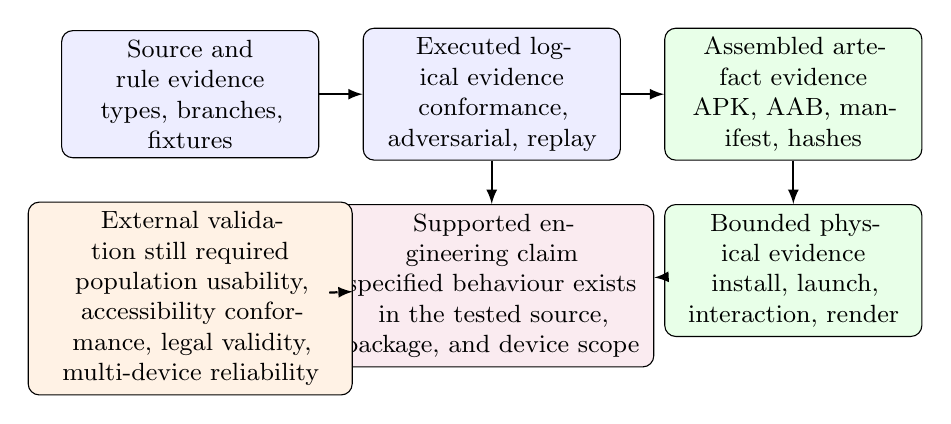
\begin{tikzpicture}[
  node distance=0.55cm,
  evidence/.style={draw, rounded corners, align=center, text width=0.25\textwidth, minimum height=1.25cm, font=\small},
  claim/.style={draw, rounded corners, align=center, text width=0.32\textwidth, minimum height=1.25cm, font=\small},
  arrow/.style={-latex, thick}
]
\node[evidence, fill=blue!7] (source) {Source and rule evidence\\types, branches, fixtures};
\node[evidence, fill=blue!7, right=of source] (tests) {Executed logical evidence\\conformance, adversarial, replay};
\node[evidence, fill=green!9, right=of tests] (package) {Assembled artefact evidence\\APK, AAB, manifest, hashes};
\node[evidence, fill=green!9, below=of package] (device) {Bounded physical evidence\\install, launch, interaction, render};
\node[claim, fill=purple!8, below=of tests] (supported) {Supported engineering claim\\specified behaviour exists in the tested source, package, and device scope};
\node[claim, fill=orange!10, below=of source] (external) {External validation still required\\population usability, accessibility conformance, legal validity, multi-device reliability};
\draw[arrow] (source) -- (tests);
\draw[arrow] (tests) -- (package);
\draw[arrow] (package) -- (device);
\draw[arrow] (tests) -- (supported);
\draw[arrow] (device) -- (supported);
\draw[dashed,-latex,thick] (supported) -- (external);
\end{tikzpicture}
\caption{Evaluation triangulation and claim boundary}
\label{fig:evaluation-triangulation}
\end{figure}

The deterministic tests and source review converge on threshold semantics. Source review identifies the pack-provided baseline, multiplier, daily threshold, burst limit, and source restrictions. Boundary assertions then test values immediately around those decision points. The fixed corpus tests varied inputs at scale. Agreement across these methods reduces the chance that the reported rule differs accidentally from the implemented one. It still does not establish that the rule is a valid legal classifier.

Runtime-boundary tests and presentation tests converge on uncertainty handling. Malformed evidence is rejected at admission, low-context evidence becomes an evidence gap, and presentation projection retains that state. This end-to-end check matters because a correct engine could be undermined if the UI translated an unknown state into reassuring copy. The tests show that selected fixtures preserve meaning through the current projection; screenshot review confirms the principal labels are visible in the rendered flow.

Build logs, output existence, checksums, manifest inspection, installed-package metadata, and physical launch converge on artefact identity. Each closes a different substitution risk. A successful Gradle message without an output file would be insufficient. A local file without a checksum could be confused after rebuilding. Source manifest facts could differ after dependency merging. An installed package could be a stale version. Reading these signals together supports the conclusion that the evaluated handset ran the recorded release candidate.

Visual review and UI-hierarchy inspection also complement each other. A screenshot shows layout, colour, clipping, and hierarchy as a person sees them. A hierarchy dump exposes text, bounds, and accessibility-node structure that may not be obvious visually. Neither replaces screen-reader interaction, large-font testing, or participant comprehension. Their combined use supports a bounded expert assessment and identifies the next accessibility evidence required.

Triangulation is not vote counting. If one authoritative check contradicts another, the discrepancy must be resolved rather than outvoted. For example, an installed-package dump showing a sensitive permission would invalidate a source-only conclusion even if several documents said otherwise. The evaluation gives greater weight to evidence closest to the released artefact for package claims and to independent human or legal review for substantive claims.

\subsubsection{Oracle Independence and Correlated Defect Risk}

The main corpus labels are derived from the same published threshold model the implementation is intended to realise. This is appropriate for conformance testing: it asks whether the program implements the specification. It is insufficient for empirical validation because a mistaken specification can yield perfect agreement. The measured 1.0000 precision and recall are therefore implementation-oracle agreement values, not estimates of performance on real legal cases.

Several design choices reduce accidental coupling. The generator records expected polarity directly from its construction, a fresh engine limits cross-case state, boundary cases are written explicitly, and extended tests target properties beyond the main daily-total rule. Nevertheless, developer knowledge shaped both sides. The campaign did not use a separately developed executable oracle, blinded labels, or an external benchmark.

Mutation testing would provide one useful next check. Deliberately changing a comparison from greater-than to greater-than-or-equal, weakening source validation, removing replay replacement, or allowing overlapping history should cause specific tests to fail. Surviving mutations would identify assertions that execute code without distinguishing correct behaviour. Property-based generation could then explore many valid and invalid shapes while preserving stated invariants.

An independent reference implementation could further reduce correlated defects. It should be written from the regulation-pack contract by a reviewer who has not read the production engine, ideally in a different language or style. Both implementations could evaluate a versioned interchange corpus. Disagreement would trigger case analysis rather than majority voting. This process would validate formal semantics, though it would still not validate legal relevance.

For legal or ecological validation, the oracle must change. Controlled event traces can provide ground truth about whether acquisition observed an action. Independent privacy reviewers can label whether a scenario warrants investigation, using a documented protocol and recording disagreement. Neither source should be described as perfect legal truth. The evaluation question, sampling frame, and annotation uncertainty must be reported alongside performance metrics.

This distinction explains why the thesis retains the term deterministic corpus rather than benchmark. A benchmark normally suggests comparison against an external reference population. The current corpus is a rigorous regression artefact that protects rule semantics as the code changes. Its value is high, but different from an independently labelled real-world set.

\subsubsection{Metric Interpretation and Error Analysis}

Precision and recall were included because they expose false-positive and false-negative cells more clearly than accuracy in an imbalanced corpus. The designed 80/20 mixture would allow a trivial always-positive strategy to appear 80 per cent accurate. The full confusion matrix prevents that reading: all 200 controls were negative and all 800 constructed signals were positive under the specified oracle.

The exact totals also make the experiment reproducible. The campaign did not sample a changing external population; it evaluated a fixed generated set. Confidence intervals around the observed proportions would describe repeated sampling from an assumed generator, not uncertainty about the fixed run. More importantly, they would not address specification validity. For this reason the report presents exact agreement and claim boundaries instead of using a narrow interval to imply real-world certainty.

Error analysis remains meaningful even when the main matrix has no disagreements. Adversarial suites reveal categories the primary generator does not represent: unsafe numeric values, prototype-derived identifiers, malformed context, source forgery, temporal overlap, replay, and history isolation. These tests show that corpus size alone is not coverage. A small, carefully targeted case can provide more security evidence than hundreds of additional values drawn from the same safe range.

Future field studies should report more than aggregate precision and recall. Results should be stratified by permission, application category, source authority, foreground status, OEM, Android version, and window resolution. Reviewers should inspect false positives and negatives for common causes. Missing acquisition records should not be treated as model negatives. Cases excluded because evidence is insufficient should be counted and explained rather than removed from the denominator without notice.

Calibration should be evaluated separately from discrimination. A status hierarchy may rank more concerning cases correctly while its displayed wording still conveys excessive certainty. Participant studies can test whether confidence changes appropriately between authoritative, synthetic, and incomplete evidence. This human calibration outcome is central to the product's trust claim and cannot be inferred from the engine matrix.

Operational metrics also need denominators. A launch success rate requires a defined number of clean starts and devices. A crash-free percentage requires a meaningful observation period and collection method. A jank percentage depends on a representative interaction trace and enough rendered frames. The current evaluation reports bounded events directly rather than producing population-style percentages from a short sample.

\subsubsection{Store-Candidate Evidence Review}

The project-defined store-candidate gate was assessed across product identity, core journey, disclosure, packaging, privacy posture, accessibility foundations, and operational ownership. Product identity was supported by a consistent name, icon, visual language, and package identifier. Core journey was supported by first-launch overview, findings navigation, detailed rationale, pack selection, demonstration control, and local-data deletion. Disclosure was supported by visible source labels, pack identity, evidence limits, and non-verdict language.

Packaging evidence included release APK and AAB generation, target SDK 36, final checksums, manifest reconciliation, signature verification, and installation of the APK. Privacy posture included no network or sensitive runtime permission in the final package, disabled backup and remote updates, local-first storage, and a release contract that scans application source for network-client APIs. Accessibility foundations included textual state labels, non-colour cues, explicit control labels and hints, selected/expanded state, a polite live region, target sizing, and a simple navigation structure.

Supply-chain review began with 30 npm findings: two critical, 17 high, ten moderate, and one low. Compatible lock-file updates plus explicit patched overrides for \texttt{brace-expansion} 1.1.18 and \texttt{postcss} 8.5.26 removed the critical findings and reduced the report to 20 findings, comprising ten high and ten moderate reports rooted in Expo/Metro build-time image parsing and Apple configuration tooling. The final Android artefact was rebuilt after the updates. This reduction is useful maintenance evidence, but it is not a zero-vulnerability claim; the remaining advisories require a separately validated Expo major transition or upstream resolution.

The gate was not interpreted as proof that every store prerequisite is complete. Production upload signing was absent. The privacy policy required owner-controlled HTTPS publication. Console declarations, listing assets, support details, content rating, internal-track delivery, and store review remained external. These gaps do not negate the engineering candidate; they determine why it must not be described as a publicly released production version.

The visual adjectives in the project gate were converted into inspectable expert-review criteria. Visual coherence meant consistent hierarchy, spacing, typography, colour restraint, branded identity, and absence of visible broken states in the inspected flows. Claim-boundary coherence meant that evidence provenance, pack governance, and limitations were prominent, destructive controls were explicit, and the product did not present a legal approval badge. Interaction feasibility meant that the evaluator could understand the purpose, navigate the product, switch and persist the review framework, and control data without a blocking defect. The resulting 95.1 score authorises the next engineering stage; none of these observations measures population preference, trust, adoption, or willingness to continue use.

These definitions create a repeatable expert gate, but they do not convert subjective judgement into population evidence. A single evaluator can miss cultural preferences, accessibility barriers, unfamiliar terminology, or long-term fatigue. The appropriate next step is internal-track and participant evaluation using the actual distributed candidate. The expert gate answers whether that investment is justified, not whether the market has accepted the product.

The candidate judgement also depends on the declared product category. A local research and accountability aid can be useful with bounded imported or simulated evidence. A product marketed as universal device surveillance would fail because the acquisition authority is not established. Store copy must preserve the former positioning. Changes to marketing are therefore capable of invalidating readiness even if the binary remains identical.

\subsubsection{Evaluation Repeatability and Change Control}

The evidence applies to a specific source revision and generated artefacts. Repeating only the final UI flow after changing engine code would not renew rule evidence. Rebuilding only the APK after changing privacy copy would not renew screenshot evidence. The project therefore treats acceptance as a dependency graph: a change invalidates every downstream artefact that incorporates or presents it.

Engine or pack changes require TypeScript compilation, logical suites, boundary suites, presentation projections, release rebuilds, hashes, and targeted device review. Android manifest or Gradle changes require merged-manifest inspection, package dump reconciliation, rebuilds, installation, and launch. UI changes require lint, package build, hierarchy and screenshot capture, accessibility checks, and renewed expert review. Policy or store-description changes require reconciliation with package behaviour and data flows.

Reproducible scripts reduce omission but do not remove the need to inspect their outputs. A command may exit successfully while testing stale generated code, selecting the wrong device, or reading a prior file. The campaign therefore compiles generated runners immediately before execution, checks package identity after installation, and associates evidence with checksums. Future automation should emit a machine-readable manifest linking commit, tool versions, commands, artefact hashes, device facts, and screenshots.

Environment details also matter. Windows path length and native dependency layout affected release compilation. The chosen workaround and architecture flag belong in the build record because a different environment may produce different outputs. Tool warnings about future Gradle compatibility remain maintenance observations even when the current build passes.

A release tag should be immutable, while packs and policies use explicit version identifiers. If a later investigation finds an error, the project should publish a successor and a correction note rather than rewriting the historical evidence. This thesis follows the same principle by creating Revision 17 chapter files instead of replacing Revision 16. Preservation makes it possible to see which claims changed and why.

Repeatability finally includes honest failure recording. Network, dependency, device-coordinate, and build-path failures can be part of the evidence because they expose operational assumptions. Removing them from the narrative would make future reproduction harder. A trustworthy evaluation explains both the final pass and the conditions needed to obtain it.

\subsection{Evaluation Synthesis}

The results answer the engineering, interface, and bounded human-factors-design portions of the Revision 17 research problem. The engine accepts and rejects the enumerated evidence classes deterministically; replay and overlap rules prevent the tested forms of aggregate amplification; pack switching changes rule-owned output without changing generic infrastructure; and legal-evidence tests preserve source status, basis-specific gaps, and non-verdict language. Renewed Android evidence connects Revision 17 source to 1.5.0 release artefacts and a bounded rendered workflow, while Revision 16 evidence remains historical rather than overwritten.

The strongest supported conclusion is therefore a versioned chain rather than a single score. Revision 17 retains the strengthened legal-evidence contract, passes current source acceptance, builds as version 1.5.0, and completes a bounded physical-device and human-factors presentation round. The chain still stops before legal adjudication, unrestricted acquisition, population performance, validated comprehension, broad usability, accessibility conformance, long-run reliability, production signing, and store approval. Chapter 6 examines why those boundaries remain material and which future evidence could move them.

\input{Iteration-V2/Chapter6/chapter-06-17}
\input{Iteration-V2/Chapter7/chapter-07-17}
{\small
\bibliographystyle{ieeetr}
\bibliography{reference}
}
\end{document}
